\chapter{Introduction}
\label{sec:intro}

\setcounter{footnote}{0}

%%%%%%%%%%%%%%%%%%%%%%%%%%%%%%%%%%%%%%%%%%%%%%%%%%%%%%%%%%%%%%%%%%%%%%%%%%%%%%%
%%%%%%%%%%%%%%%%%%%%%%%%%%%%%%%%%%%%%%%%%%%%%%%%%%%%%%%%%%%%%%%%%%%%%%%%%%%%%%%

Thermodynamics originated as the study of heat and its transformations into other
forms of energy, but can more generally be described as the study of bulk matter.
That is, it seeks to answer questions regarding those properties of matter that
are defined in terms of large collections of particles. Two
familiar examples are density and temperature. The density of a substance is
its mass per unit volume.
Such a quantity is sometimes said to be \emph{intensive}: it depends only on
the nature of the substance under consideration, not on the amount that is present.

There is a small caveat that should be added to this definition: the mass per unit
volume of a sample of some substance will only become independent of the volume once
this volume is sufficiently large. This makes density a \emph{macroscopic} quantity
(as opposed to, e.g.\ the atomic number). To say that thermodynamics is the study
of bulk matter amounts to saying that it deals in macroscopic quantities.
% Thus, it does not make sense to ask for the density of a sample of hydrogen consisting
% of a single atom although it is sensible to speak of the density of hydrogen.
% In this sense, density is not
% only a true property of the substance, but in fact a \emph{macroscopic} property
% (as opposed to, e.g.\ the atomic number of hydrogen) and thermodynamics is the
% study of macroscopic properties.

% The fact that there is such a distinction between microscopic and macroscopic
% properties raises a number of simple questions.
This raises a number of simple questions. For instance, if these quantities
are truly intensive, then it should be possible to 
derive them from the microscopic behaviour of the substance's constituent particles;
yet above, we have resorted to discussing ``large'' quantities of matter in order
to make sense of density. In fact, this leads us to another natural question: what
constitutes a sample sufficiently large to be considered bulk matter and why should
certain measurements of a sample stabilize when the sample is large?

A natural response is that some sort of law of large numbers
must be at work. Although the behaviour of a system of particles is not random, it may
be sufficiently complex that it is reasonable to view it as such.
This is the basic idea of equilibrium statistical mechanics: to leverage the complexity of
large systems of particles in order to explain the apparent simplicity of bulk
matter as arising from the kind of self-averaging that pervades probability
theory. From this point of view, macroscopic quantities are types of averages that
arise from some probability distribution. These averages typically depend on
temperature or other parameters, so in this sense the main objects of study in
statistical mechanics are certain parameterized families of probability measures.

It is useful to organize these measures according to their qualitative properties.
Qualitatively similar measures correspond to a \emph{phase} of a substance. For
instance, water at $20^\circ{\rm C}$ is not significantly different from water at
$50^\circ{\rm C}$. On the other hand, steam and water have very different behaviours
despite both being $\mathrm{H_2O}$. In fact, the boiling of water is signalled by an
abrupt drop in density by a factor of around $1/1000$ at normal atmospheric pressure.

A similar effect occurs under different atmospheric conditions as well. The temperature
at which water
boils varies as a function of pressure $T_c = T_c(P)$ and a \emph{phase transition}
is said to occur when the pressure and/or temperature are varied in such a way as to
cross the graph of this function; see Figure~\ref{fig:liquid-vapour}.
However, as $P$ is increased, the density difference along this curve decreases and
there is a \emph{critical point} $(T_c(P_c), P_c)$ at which this difference vanishes.

\begin{figure}
\centering
\label{fig:liquid-vapour}
\includegraphics{liquid_vapour}
\caption[Phase diagram of $\rm H_2 O$]{The phase diagram of $\rm H_2 O$}
\end{figure}

Since statistical mechanics deals with extremely large, complicated systems of
interacting particles, only simplified models of real materials can usually be
studied in detail. Such models are useful for building a
\emph{qualitative} understanding of the phases of matter and phase transitions.
However, the simplifications inherent in their definitions mean that they are
usually not suitable for making quantitative predictions.

A remarkable phenomenon, known as \emph{universality}, is that this is no longer
entirely true at the critical point. At criticality, many quantities behave in a
way that is independent of the fine details of the model being used. Thus,
some of the \emph{quantitative} properties of real materials can in principle be
predicted exactly by studying models only roughly resembling these materials
% is in their very coarse properties.

In the 1970's Ken Wilson, inspired by ideas in quantum field theory, gave an
explanation of universality in terms of the \emph{renormalisation group}:
an abstract dynamical system that acts on models by averaging out their fine details.
This idea was enormously successful and led to his 1982 Nobel Prize.

Nevertheless, a mathematically rigorous understanding of the renormalisation group
remains incomplete. Although there have been several rigorous implementations of
Wilson's ideas, they tend to be highly technical and restricted to somewhat special
classes of models. The main purpose of this thesis is to discuss extensions of a
rigorous renormalisation group method of Bauerschmidt, Brydges, and Slade that have
been used to study the
critical behaviour of a generalized $|\varphi|^4$ model and a model of weakly
self-avoiding walk with contact self-attraction (WSAW-SA). We will introduce these
models and our main results in the present chapter and discuss the proofs in the
remainder of the thesis.

We begin in Section~\ref{sec:asymp} with some general background on asymptotic
notation and the method of generating functions and Laplace transforms. In
Section~\ref{sec:gibbs}, we briefly introduce some of the basic ideas of equilibrium
statistical physics. The models we study are defined on graphs, which we
discuss in Section~\ref{sec:graphs}. We define spin systems, in particular
the $|\varphi|^4$ model, in Section~\ref{sec:spins}. Critical behaviour and
the renormalisation group is probably most easily explained in the context of such
systems, and we give an informal description of these ideas in Section~\ref{sec:crit}.
In Section~\ref{sec:walks},
we introduce the WSAW-SA and discuss its critical behaviour. This gives us all
the necessary definitions to state our main results in Section~\ref{sec:mr}.
Before proceeding to the method of proof,
we discuss the close relationship between models of walks and spin systems in
Section~\ref{sec:spin-walk}; in particular, we recall a representation
of the WSAW-SA in terms of a spin system related to the $|\varphi|^4$ model
that allows us to unify our treatment of both models.

%%%%%%%%%%%%%%%%%%%%%%%%%%%%%%%%%%%%%%%%%%%%%%%%%%%%%%%%%%%%%%%%%%%%%%%%%%%%%%%
%%%%%%%%%%%%%%%%%%%%%%%%%%%%%%%%%%%%%%%%%%%%%%%%%%%%%%%%%%%%%%%%%%%%%%%%%%%%%%%

\section{Asymptotics}
\label{sec:asymp}

We begin by with a short discussion of some useful notation and mathematical
background.

%%%%%%%%%%%%%%%%%%%%%%%%%%%%%%%%%%%%%%%%%%%%%%%%%%%%%%%%%%%%%%%%%%%%%%%%%%%%%%%

\subsection{Asymptotic notation}

Let $F$ and $G$ be a functions on a subset of the real line.
For $a\in[-\infty,\infty]$, we write
\begin{alignat}{2}
F(x) &\sim G(x), &&\qquad x \to a \\
F(x) &= o(G(x)), &&\qquad x \to a
\end{alignat}
if, respectively,
\begin{align}
&\lim_{x\to a} \frac{F(x)}{G(x)} = 1 \\
&\lim_{x\to a} \frac{F(x)}{G(x)} = 0.
\end{align}
We also write
\begin{equation}
F(x) = O(G(x))
	\text{ or }
F(x) \le O(G(x)),
	\qquad
x \to a
\end{equation}
if there is a constant $C \ge 0$ such that $|F(x)| \le C G(x)$ for all
$x$ in some neighbourhood of $a$ (in the extended real line). Lastly, we write
\begin{equation}
F(x) \asymp G(x),
	\qquad
x \to a
\end{equation}
if $F(x) = O(G(x))$ and $G(x) = O(F(x))$ as $x\to a$, possibly with
different constants for the two inequalities. We will sometimes write
$F(x) \approx G(x)$ in heuristic
arguments where the hope is that a rigorous argument might replace $\approx$
by $\asymp$ or $\sim$.

%%%%%%%%%%%%%%%%%%%%%%%%%%%%%%%%%%%%%%%%%%%%%%%%%%%%%%%%%%%%%%%%%%%%%%%%%%%%%%%

\subsection{Generating function and Laplace transform}

The \emph{generating function} of a sequence $a_n$ is the function $g(z)$ defined
by the power series with coefficients $a_n$:
\begin{equation}
g(z) = \sum_{n=0}^\infty a_n z^n.
\end{equation}
If the function $g$ is sufficiently well understood, then the coefficients
can be recovered by differentiation:
\begin{equation}
a_n = \frac{1}{n!} g^{(n)}(0).
\end{equation}
This is known as the method of generating functions \cite{Wilf06}.

In many cases, $g$ cannot be computed exactly. Nevertheless, there is a close
relationship between the asymptotics of the sequence $a_n$
as $n\to\infty$ and the function $g(z)$ near its dominant singularities, i.e.\
its singularities closest to the origin \cite{FS09}.
For instance, if $a_n \sim r^{-n} n^\alpha$, then the root test implies that
the generating function $f$ has radius of convergence $r$. If, moreover, $a_n \ge 0$,
then $g(z) \sim C (r - z)^{-(\alpha+1)}$ as $z \uparrow r$.		% See Madras-Slade
This is an
example of an \emph{Abelian theorem}. The converse does not always hold; a
theorem providing conditions under which the converse is true is known as a
\emph{Tauberian theorem}, and is generally harder to prove than its Abelian
counterpart.

% \commentbw{See Feller Vol II, Chap XIII, Section 5}

Likewise, the asymptotics of a function $f(T)$ as $T\to\infty$ can sometimes
be recovered from the behaviour of its \emph{Laplace transform}
\begin{equation}
\label{e:laplace-transform-def}
G(\nu) = \int f(T) e^{-\nu T} \; dT
\end{equation}
near $\nu_0 \coloneqq \inf \{ \nu : G(\nu) < \infty \}$.
There are Abelian and Tauberian theorems for the Laplace transform analogous
to those for generating functions. For instance,
$f(T) \sim A T^\alpha$ implies that $G(\nu) \sim A' (\nu - \nu_0)^{-(\alpha+1)}$
as $\nu\downarrow\nu_0$ and the converse holds when $f$ is monotone (see \cite{Widd41}).

% For instance, we have the following (see \cite[Chapter V]{Widd41}).
% 
% \begin{theorem}
% Suppose that there exist $\nu_0$ such that
% the function $G(\nu)$ defined by \eqref{e:laplace-transform-def} converges for
% $\nu > \nu_0$. If there exist $A$ and $\alpha \ge 0$ such that
% \begin{equation}
% f(T) \sim \frac{A}{\Gamma(\alpha + 1)} T^\alpha,
% \end{equation}
% then
% \begin{equation}
% G(\nu) \sim A \nu_0 (\nu - \nu_0)^{-(\alpha+1)}.
% \end{equation}
% Moreover, the converse holds if $f(T)$ is increasing.
% \end{theorem}
% 
% When $f$ is not monotonic, it may still be possible to recover its asymptotic
% behaviour from $G$ by inverting the Laplace transform. However, control over
% $G$ for $\nu$ in a sector of the complex plane is required in this case.

%%%%%%%%%%%%%%%%%%%%%%%%%%%%%%%%%%%%%%%%%%%%%%%%%%%%%%%%%%%%%%%%%%%%%%%%%%%%%%%
%%%%%%%%%%%%%%%%%%%%%%%%%%%%%%%%%%%%%%%%%%%%%%%%%%%%%%%%%%%%%%%%%%%%%%%%%%%%%%%

\section{Equilibrium statistical mechanics}
\label{sec:gibbs}

Let $(\Omega, \lambda)$ be a measure space. We view $\lambda$ as some ``natural''
measure on $\Omega$. The dynamics of a physical system with state space $\Omega$
are often determined by a function $H$ on $\Omega$, known as the \emph{Hamiltonian}.
Typically, $H(\omega)$ represents the total energy of the system in state $\omega$;
it is thus reasonable to assume that $H$ is bounded below\footnote{It is convenient
to allow $H$ to take on negative values.}.

\begin{example}
\label{ex:hamilton}
The canonical example is a system of $n$ point particles in a domain $U \subset \R^3$,
for which $\Omega = (U \times \R^3)^n$ and $\lambda$ is Lebesgue measure on $\Omega$.
A state $\omega\in\Omega$ consists of the positions $q_i \in U$ and momenta $p_i \in \R^3$
of the $n$ particles. The Hamiltonian is usually smooth and the dynamics are determined
by Hamilton's equations
\begin{align}
\dd{q}{t} 	&= \nabla_p H \\
-\dd{p}{t} 	&= \nabla_q H.
\end{align}
Typically, the Hamiltonian has the form
\begin{equation}
\label{e:total-energy}
H(q, p) = \frac{1}{2m} |p|^2 + U(q).
\end{equation}
The first term is the usual definition of kinetic energy and the second term,
which depends only on $q$, is a potential energy function.
\end{example}

In statistical mechanics, the systems of concern consist of a very large number
of particles ($n$ large in the previous example). Typically, the state space
$\Omega$ is very high-dimensional and studying the exact dynamics is infeasible.

A common simplifying assumption is that after a long time has passed, the system
will settle into a state of \emph{thermal equilibrium}, meaning that there is no
net flow of heat between the system and its surroundings. Thus, the temperature is
constant; we denote by $\beta$ the \emph{inverse temperature}. The \emph{Gibbs measure} %\cite{Gibbs60}
for a system with Hamiltonian $H$ at inverse temperature
$\beta$ is the probability measure on $\Omega$ given by
\begin{equation}
\label{e:gibbs-def}
\mu_\beta(d\omega) = \frac{1}{Z} e^{-\beta H(\omega)} d\lambda(\omega)
\end{equation}
when this is well-defined.
The normalizing constant
\begin{equation}
Z = \int e^{-\beta H} \; d\lambda
\end{equation}
is known as the \emph{partition function}.

% A simple approach to the derivation of this measure was suggested by Jaynes \cite{Jaynes57}:
% under appropriate hypotheses, amongst all probability measures $\mu$ on $\Omega$ absolutely
% continuous with respect to $\lambda$, the Gibbs measure maximizes the \emph{entropy}
% \begin{equation}
% \label{e:entropy-def}
% \entropy(\mu) = -\int \log \frac{d\mu}{d\lambda} \; d\mu
% \end{equation}
% with respect to $\lambda$, subject to the fixed average energy constraint
% \begin{equation}
% \label{e:fix-avg-energy}
% \int H \; d\mu = E.
% \end{equation}
% This can be shown using the method of Lagrange multipliers;
% the parameter $\beta = \beta(E)$ arises as a Lagrange multiplier.

%%%%%%%%%%%%%%%%%%%%%%%%%%%%%%%%%%%%%%%%%%%%%%%%%%%%%%%%%%%%%%%%%%%%%%%%%%%%%%%

\subsection{Relation to quantum theory}
\label{sec:quantum}

Let us briefly describe the relationship between equilibrium statistical
mechanics and quantum field theory. Our presentation is heuristic and involves
manipulations of a priori ill-defined objects. A rigorous development of these
ideas goes back to \cite{Syma69,Nelson73,OS73,OS75}; useful references are
\cite{Simon05} (for quantum mechanics) and \cite{GJ87} (for quantum
field theory).

Let $H(x, p)$ be the Hamiltonian \eqref{e:total-energy} (we have written $x$
instead of $q$). In quantum mechanics, the state space is replaced by a Hilbert
space, usually $L^2 = L^2(\R^{3n})$;
the position $x_j$ is replaced by the \emph{position operator} $\hat x_j$ given by
multiplication by $x_j$; and the momentum $p_j$ is replaced by the \emph{momentum
operator} $\hat p_j = -i \hbar \partial/\partial x_j$ (we ignore details regarding
the domains of these operators). The resulting operator $\hat H = H(\hat x, \hat p)$
on $L^2$ determines the evolution of the \emph{wave function} $\psi\in L^2$ via
the Schr\"{o}dinger equation
\begin{equation}
i\hbar \dd{\psi}{t} = \hat H \psi
\end{equation}
whose solution with initial condition $\psi(0)$ is given by
$\psi(t) = e^{-it\hat H/\hbar} \psi(0)$.

Suppose that the solution operator is an integral operator with kernel $K_t$:
\begin{equation}
e^{-it\hat H/\hbar} f = \int K_t(\cdot, y) f(y) \; dy.
\end{equation}
The Feynman path integral formulation of quantum mechanics \cite{Feyn48}
involves writing the kernel as
\begin{equation}
K_t(a, b)
	=
\int_{\cwalks_t(a, b)} e^{(i/\hbar) \int_0^t L(x(s), \dot x(s)) \; ds} \; \Dcal x,
\end{equation}
where $\cwalks_t(a, b)$ is a space of paths $[0, t] \to \R^{3n}$ from
$a$ to $b$ equipped with a ``Lebesgue measure'' $\Dcal x$ and
\begin{equation}
L(x, \dot x) = \frac{1}{2} m |\dot x|^2 - U(x)
\end{equation}
is the \emph{Lagrangian} of the classical system we started with.
As such, the integral representation of $K_t$ is ill-defined;
for instance, the measure $\Dcal x$ on paths does not exist. However, let us
not concern ourselves with this.

Suppose that $\psi$ can be analytically continued to a region of the complex
plane containing the positive imaginary axis. Then we might hope the function
$t \mapsto \psi(-it)$ has solution operator with kernel of the form
\begin{equation}
K_{-it}(a, b)
	=
\int_{\cwalks_{-it}(a, b)} e^{(i/\hbar) \int_0^{-it} L(x(s), \dot x(s)) \; ds} \; \Dcal x.
\end{equation}
By the change of variables $s = -iu$,
\begin{equation}
(i/\hbar) \int_0^{-it} L(x(s), \dot x(s)) \; ds
	=
(1/\hbar) \int_0^t L(\tilde x(u), i \dot{\tilde x}(u)) \; du
	=
-(1/\hbar) \int_0^t H(\tilde x(u), m \dot{\tilde x}(u)) \; du
\end{equation}
with $\tilde x(t) = x(-it)$. Thus, by the fictive change of variables in which
$\cwalks_{it}(a, b)$ is replaced by $\cwalks_t(a, b)$, we get
\begin{equation}
\label{e:heat-kernel-fake}
K_{-it}(a, b)
	=
\int_{\cwalks_t(a, b)} e^{-(1/\hbar) \int_0^t H(x(u), m\dot x(u)) \; du} \; \Dcal x
\end{equation}
This procedure is known as a \emph{Wick rotation}.

The analogue of this idea in quantum field theory involves replacing integration
over paths with integration over fields $\varphi$, which are functions on $\Rd$.
The corresponding ``measures'' of the form $e^{-(1/\hbar)\int H} \Dcal\varphi$
should be compared with the Gibbs measures \eqref{e:gibbs-def} with Planck's constant
$\hbar$ playing the role of temperature. Although $H$
has been replaced by the \emph{integral} $\int H$, we will discuss how natural
choices for the Hamiltonian in a Gibbs measure are given by \emph{sums} over
spaces of fields on discrete approximations to $\Rd$ (graphs).

\begin{rk}
In fact, it turns out that \eqref{e:heat-kernel-fake} is not too unreasonable.
For simplicity, let us take $\hbar = 1$ and $m = 1$.
Then we would expect $\tilde\psi$ to solve
\begin{equation}
\label{e:linear-pde}
\dd{\tilde\psi}{t} = -\hat H \tilde\psi.
\end{equation}
When $U = 0$, we have $H(x, p) = |p|^2$, so $\hat H = -\tfrac12 \Delta_{\R^{3n}}$
is the Laplacian on $\R^{3n}$ and \eqref{e:linear-pde} is the heat equation.
On the other hand, $\int_0^t H$ is formally a positive-definite quadratic form, so
\eqref{e:heat-kernel-fake} is a formal Gaussian integral. This is consistent
with the well-known fact that a solution $\tilde\psi$ of the heat equation
on a domain can (under appropriate conditions) be written as
$\tilde\psi(t, x) = \Ex(\tilde\psi(0, B_t) \mid B_0 = x)$,
where $B_t$ is a Brownian motion.
More generally, under appropriate hypotheses, the Feynman-Kac formula expresses
solutions to \eqref{e:linear-pde} with $U \ne 0$ as averages with respect to a
Brownian motion.
\end{rk}

%%%%%%%%%%%%%%%%%%%%%%%%%%%%%%%%%%%%%%%%%%%%%%%%%%%%%%%%%%%%%%%%%%%%%%%%%%%%%%%
%%%%%%%%%%%%%%%%%%%%%%%%%%%%%%%%%%%%%%%%%%%%%%%%%%%%%%%%%%%%%%%%%%%%%%%%%%%%%%%

\section{Graphs}
\label{sec:graphs}

An \emph{undirected graph} or simply a \emph{graph} is a pair $\graph = (\vertices, \edges)$,
where $\vertices$
is a set of \emph{vertices} and $\edges$ is a set of
\emph{edges} $\{ x, y \}$ with $x, y \in \vertices$; we will write $x \sim y$ if
$\{ x, y \} \in \edges$.
For simplicity, we will assume that $\vertices$ is countable and that there are no
\emph{self-loops} $\{ x \} \in \edges$.

A graph \emph{automorphism} is a function $f : \vertices\to\vertices$ such that
$x \sim y$ if and only if $f(x) \sim f(y)$.
We will assume that $\graph$ is \emph{transitive} meaning that for all pairs
of distinct
vertices $a, b \in \vertices$, there exists an automorphism $f$ with $f(a) = b$.
We fix a vertex $0\in\vertices$ whose precise choice is immaterial due to
transitivity.

%%%%%%%%%%%%%%%%%%%%%%%%%%%%%%%%%%%%%%%%%%%%%%%%%%%%%%%%%%%%%%%%%%%%%%%%%%%%%%%

\subsection{Functions on graphs}

Let us denote the components of an element $\varphi \in (\R^n)^\vertices$ by
$\varphi^i_x \in \R$ for $x \in \vertices$ and $i = 1, \ldots, n$.
The Euclidean inner product and norm on $(\R^n)^\vertices$
are defined by
\begin{align}
\varphi\cdot\tilde\varphi
	&= \sum_{x\in\vertices} \varphi_x \cdot \tilde\varphi_y
  		= \sum_{i=1}^n \sum_{x\in\vertices} \varphi^i_x \tilde\varphi^i_x \\
|\varphi|^2
	&= \varphi \cdot \varphi.
\end{align}
A $\vertices\times\vertices$ matrix $M = (M_{xy})_{x,y\in\vertices}$ acts on $\varphi$
component-wise:
\begin{equation}
(M \varphi)_x = \sum_{y\in\vertices} M_{xy} \varphi_y.
\end{equation}

%%%%%%%%%%%%%%%%%%%%%%%%%%%%%%%%%%%%%%%%%%%%%%%%%%%%%%%%%%%%%%%%%%%%%%%%%%%%%%%

\subsection{The graph Laplacian}

Let us say that a $\vertices\times\vertices$ matrix $M$ is \emph{indexed by} $\edges$
if $M_{xy} \ne 0$ if and only if $x \sim y$.
Throughout this chapter, we let $\jay$ be a matrix indexed by $\edges$ with nonnegative entries.
Thus,
\begin{equation}
\jay_{xy} \ge 0
\end{equation}
with equality if and only if $x \not\sim y$.
The pair $(\graph, \jay)$ is an example of a \emph{weighted} graph.
We will usually denote this weighted graph simply as $\graph$, with $\jay$
implicit.

Let $\diag$ be the diagonal $\vertices\times\vertices$ matrix with diagonal entries
\begin{equation}
d_x = \diag_{xx} = \sum_{y \sim x} J_{xy},
\end{equation}
where the sum is over all vertices $y$ adjacent to $x$.
% We say that $\graph$ is \emph{$d_0$-regular} if $d_x = d_y$ for all $x, y$.
The graph \emph{Laplacian} on $\graph$ is defined by
\begin{equation}
-\lap = \diag - \jay.
\end{equation}
An important case is when $\jay_{xy} = \1_{x\sim y}$, for which
\begin{equation}
\label{e:Deltaxy}
-\Delta_{xy} = d_x \1_{x=y} - \1_{x \sim y}.
\end{equation}
We also define the \emph{massive Laplacian} with squared \emph{mass} $m^2 > 0$ by
\begin{equation}
-\lap + m^2.
\end{equation}
Note that
\begin{equation}
\label{e:sbp-gen}
\varphi \cdot (-\lap \varphi)
  =
\frac{1}{2} \sum_{x,y\in\vertices} J_{xy} |\varphi_x - \varphi_y|^2
  \ge
0,
\end{equation}
so $-\lap$ is positive-semidefinite.

\begin{example}
We will often work on the discrete $d$-dimensional \emph{torus}
of side $L^N$, defined by
\begin{equation}
\label{e:Lambda-torus}
\Lambda = \Lambda_N = \Zd/L^N\Zd
\end{equation}
for integers $L > 1$ and $N \ge 0$.
We view $\Lambda$ as a graph with $\vertices = \Lambda$ and $x \sim y$ if
$x$ and $y$ have distance $1$ on the torus. This graph is transitive
and $d_x = 2d$ for all $x$.
\end{example}

%%%%%%%%%%%%%%%%%%%%%%%%%%%%%%%%%%%%%%%%%%%%%%%%%%%%%%%%%%%%%%%%%%%%%%%%%%%%%%%

\subsection{The Green function}

If $m^2 > 0$, then $-\lap + m^2$ is positive-definite, hence invertible with inverse
\begin{equation}
(-\lap + m^2)^{-1} = (m^2 + D)^{-1} \sum_{n=0}^\infty Z^n P^n,
\end{equation}
where
\begin{equation}
Z = (m^2 + D)^{-1} D,
  \quad
P = D^{-1} J.
\end{equation}
Let $z_x$ denote the diagonal elements of $Z$. The \emph{Green function}
of $\graph$ is the kernel of $(-\lap + m^2)^{-1}$, given by
\begin{equation}
\label{e:greendef}
C_{xy}
  =
(m^2 + d_x)^{-1} \sum_{n=0}^\infty z_x^n P^n_{xy}.
\end{equation}

%%%%%%%%%%%%%%%%%%%%%%%%%%%%%%%%%%%%%%%%%%%%%%%%%%%%%%%%%%%%%%%%%%%%%%%%%%%%%%%
%%%%%%%%%%%%%%%%%%%%%%%%%%%%%%%%%%%%%%%%%%%%%%%%%%%%%%%%%%%%%%%%%%%%%%%%%%%%%%%

\section{Spin systems}
\label{sec:spins}

We begin by restricting our attention to spin systems in \emph{finite} volume:
\begin{equation}
|\vertices| < \infty.
\end{equation}
Suppose that $S \subset \R^n$ is equipped with a measure $d\lambda^0$, let
$\Omega = S^\vertices$, and define the product measure
\begin{equation}
d\lambda(\varphi) = \prod_{x\in\vertices} d\lambda^0(\varphi_x),
	\quad
\varphi\in\Omega.
\end{equation}
We refer to the elements of $\Omega$ as \emph{fields}
or \emph{spin configurations} on $\vertices$ with spins in $S$.

Let $H : \Omega \to \R$ be a function and suppose
that $e^{-H}$ is integrable with respect to $d\lambda$.
The \emph{spin system} with Hamiltonian $H : \Omega \to \R$
at inverse temperature $\beta$ is given by the Gibbs measure
\begin{equation}
\label{e:gibbs-spin}
d\mu_\beta(\varphi)
	=
\frac{1}{Z_\beta} e^{-\beta H(\varphi)} \; d\lambda(\varphi).
\end{equation}
We sometimes add an \emph{external field} $h \in \R$ by considering the measure
\begin{equation}
\label{e:gibbs-spin-ext}
d\mu_{\beta,h}(\varphi)
	=
\frac{1}{Z_{\beta,h}}
e^{-\beta \big(H(\varphi) - h \sum_{x\in\vertices} \varphi_x\big)} \; d\lambda(\varphi).
\end{equation}
We will mainly be concerned with \emph{ferromagnetic} spin systems, for which the
Hamiltonian is given by
\begin{equation}
H(\varphi) = -\varphi \cdot M\varphi,
	\quad
M_{xy} \ge 0.
\end{equation}
The total energy of such a system is a sum of contributions
of the form $-2 \varphi_x \cdot M_{xy} \varphi_y$ for $x \sim y$. Such a
contribution
attains its minimum when $\varphi_x = \varphi_y$ and its maximum when
$\varphi_x = -\varphi_y$. In this sense, it is energetically favourable
for spins to \emph{align} in ferromagnetic systems.

%%%%%%%%%%%%%%%%%%%%%%%%%%%%%%%%%%%%%%%%%%%%%%%%%%%%%%%%%%%%%%%%%%%%%%%%%%%%%%%

\subsection{Examples of spin systems}

Below we discuss some common examples of spin systems.
In many cases, we discuss Hamiltonians that depend on one or more parameters
for which adjusting the inverse temperature $\beta$ is equivalent to rescaling
these parameters. In these cases, we will fix
\begin{equation}
\label{e:beta-one}
\beta = 1
\end{equation}
without loss of generality.

\subsubsection{Gaussian measures}

Suppose $S = \R^n$ and $\lambda^0$ is Lebesgue measure. Then the Hamiltonian
$H$ must be bounded below for the Gibbs measure \eqref{e:gibbs-spin} to be
well-defined. Essentially the simplest class of
non-constant\footnote{The Gibbs measure with constant Hamiltonian is just the
product measure.} Hamiltonians
are positive-definite quadratic forms. These are given by a positive-definite
symmetric $\vertices\times\vertices$ matrix $C$, called the \emph{covariance}
matrix, and take the form
\begin{equation}
H_C(\varphi) = \frac{1}{2} \varphi \cdot C^{-1} \varphi.
\end{equation}
The corresponding Gibbs measures are \emph{Gaussian} measures.

The partition function can be computed explicitly and the Gibbs measure takes
the form
\begin{equation}
\label{e:gauss-density}
\frac{d\varphi}{\sqrt{\det(2\pi C)}}
e^{-\tfrac12 \varphi \cdot A \varphi}.
\end{equation}
\emph{Wick's theorem} gives an expression for the moments:
if $x_1, \ldots, x_{2p} \in \Lambda$, then
\begin{equation}
\label{e:wick}
\int d\mu_C(\varphi) \prod_{k=1}^{2p} \varphi^i_{x_k}
	=
\sum_\pi \prod_{kl\in\pi} C_{x_kx_l}
\end{equation}
where the sum is over all pairings $\pi$ of $\{1,\ldots,2p\}$ (i.e.\ partitions of
this set into $2$-element subsets).

\subsubsection{The $|\varphi|^4$ model}

As in the previous example, let $S = \R^n$ and $\lambda^0$ be Lebesgue measure.
The next step up in complexity is a quartic Hamiltonian. In particular, we have
the Hamiltonian for the \emph{lattice $|\varphi|^4$ model} or \emph{Ginzburg-Landau-Wilson model}:
\begin{equation}
\label{e:phi4-Ham}
H_{\gcc,\nu}(\varphi)
  =
\sum_{x\in\vertices}
\left(
  \frac{1}{4} \gcc |\varphi_x|^4
    +
  \frac{1}{2} \nu |\varphi_x|^2
    +
  \frac{1}{2} \varphi_x \cdot (-\lap \varphi)_x
\right),
\end{equation}
where $\gcc > 0$ and $\nu\in\R$.
The expression \eqref{e:phi4-Ham} should be compared with \eqref{e:total-energy}.
With $p = m \dot q$ in the latter expression, the kinetic energy takes the form
$\tfrac12 m |\dot q|^2$. The lattice analogue of this quantity in \eqref{e:phi4-Ham} is
\begin{equation}
\label{e:discrete-kinetic}
\frac12 \sum_{x\in\vertices} \varphi_x \cdot (-\lap \varphi)_x
	=
\frac14 \sum_{x\in\vertices} \sum_{y\sim x} (\varphi_y - \varphi_x)^2,
\end{equation}
where we have applied \eqref{e:sbp-gen} to get the right-hand side.

\begin{example}[The GFF]
With $g = 0$ and $\nu > 0$,
\begin{equation}
H_{0,\nu}(\varphi) = H_C(\varphi),
	\qquad
C = (-\lap + \nu)^{-1}.
\end{equation}
In other words, the $|\varphi|^4$ model becomes the Gaussian measure with covariance given
by the massive Green function. The corresponding spin system is the discrete massive
\emph{Gaussian free field} or \emph{GFF}.

The continuum analog of this model with mass $0$
(which can be defined on $\Rd$ with $d > 2$) is a simple example of a
non-interacting\footnote{The corresponding classical model only involves the kinetic term
\eqref{e:discrete-kinetic}.} quantum field theory. The $|\varphi|^4$ model was introduced
in attempts to construct an \emph{interacting} theory.
\end{example}

\subsubsection{The $O(n)$ spin model}

Consider the $|\varphi|^4$ model and suppose that $\sum_{y\sim x} J_{xy} = d_0$
for all $x\in\vertices$ (e.g.\ this occurs in the setting of \eqref{e:Deltaxy} when every
vertex in $\graph$ has $d_0$ neighbours).
% \begin{equation}
% d_x = \diag_{xx} = \sum_{y \sim x} J_{xy}.
% \end{equation}
% when $\graph$ is $d_0$-regular.
In this case, we can write
\begin{equation}
\label{e:phi4-split}
H_{\gcc,\nu}(\varphi)
  =
\sum_{x\in\vertices} U_{\gcc,\nu}(\varphi_x) - \frac{1}{2} \varphi \cdot \jay \varphi,
\end{equation}
where the \emph{single-spin potential} $U_{\gcc,\nu}$ is given by
\begin{equation}
U_{\gcc,\nu}(t)
	=
\frac{1}{4} \gcc |t|^4
	+
\frac{1}{2} (\nu + d_0) |t|^2,
	\quad
t \in \R^n.
\end{equation}
We can see from \eqref{e:phi4-split} that the $|\varphi|^4$ model is ferromagnetic.
When $\nu + d_0 < 0$, the potential has the shape of a double well with roots at
$t = 0$ and on the sphere $|t| = \pm\sqrt{-2 (\nu + d_0) / \gcc}$.
Thus, as $\gcc\to\infty$ with $\nu = -(d_0 + \gcc/2)$, the Gibbs measure for the
$|\varphi|^4$ model converges (weakly) to the Gibbs measure with Hamiltonian
\begin{equation}
\label{e:on-model}
H_J(\varphi) = -\frac12 \varphi \cdot J \varphi,
	\quad
\varphi \in (S^{n-1})^\vertices
\end{equation}
where $S^{n-1} \subset \R^n$ is the $(n-1)$-dimensional unit sphere.
This is known as the \emph{$O(n)$ spin model}. The special case $n = 1$ is the
famous \emph{Ising model}. The cases $n = 2$ and $n = 3$ are known as the
\emph{XY model} and the \emph{classical Heisenberg model}.

\begin{rk}
The Ising model on $\Zd$ (defined by a limiting procedure) was introduced
by Willhelm Lenz \cite{Lenz20}. Lenz
suggested it as a problem for his student Ernst Ising, who determined in 1924
\cite{Ising25} that there is no (non-trivial) phase transition when $d = 1$.
In \cite{Heisenberg28} Heisenberg, seeking a model that would possess a phase
transition, proposed the quantum version of his model (see \cite{Brush67} for
a discussion on this). Ironically, it turns out that the classical version of
his model does not possess a phase transition in both $d = 1$ and $d = 2$ \cite{MW66};
and, moreover, in 1936 Rudolf Peierls \cite{Peierls36} put forth an argument for the
existence of a phase transition in the Ising model if $d > 1$. Peierls' argument
was made rigorous in \cite{Griffiths64}, but even before that Onsager \cite{Onsager44}
provided an exact computation of the free energy in $d = 2$, which incontrovertibly
demonstrated the existence of a phase transition in two dimensions. The general
$O(n)$ model was first studied in \cite{Stanley68}.
\end{rk}

%%%%%%%%%%%%%%%%%%%%%%%%%%%%%%%%%%%%%%%%%%%%%%%%%%%%%%%%%%%%%%%%%%%%%%%%%%%%%%%

\subsection{Phase transition in the Ising model}

% In this section we discuss the phase transition for the Ising model on $\Zd$
% with $d > 1$. A good reference is \cite{FV17}.

Let $\graph = \Lambda_N$ and consider the Hamiltonian for the Ising model with
interaction $J_{xy} = \1_{x\sim y}$ in an external field $h\in\R$:
\begin{equation}
H^{(N)}_h(\varphi)
	=
-\frac12 \sum_{x \sim y} \varphi_x \varphi_y
- h \sum_{x\in\vertices} \varphi_x,
	\qquad
\varphi\in\{\pm1\}^\vertices.
\end{equation}
Let $\langle\cdot\rangle^{(N)}_{\beta,h}$ denote the expectation with respect to
the corresponding Gibbs measure $\mu^{(N)}_{\beta,h}$ and let $Z^{(N)}_{\beta,h}$
be the partition function.

The \emph{free energy} is defined (in finite volume) by
\begin{equation}
F^{(N)}_{\beta,h}
	=
-\frac{1}{\beta |\vertices|} \log Z^{(N)}_{\beta,h}.
\end{equation}
% Notice that with $h = 0$ a computation of the entropy $\entropy(\mu^{(N)}_{\beta,0})$
% with $\beta = \beta(E)$ (as in \eqref{e:fix-avg-energy}) shows that
% \begin{equation}
% F^{(N)}_{\beta,0} = E - \frac{1}{\beta} \entropy(\mu^{(N)}_{\beta,0}),
% \end{equation}
% which recovers the usual definition of Helmholtz free energy in thermodynamics.
The \emph{magnetization} is given by
\begin{equation}
M^{(N)}_{\beta,h}
	=
\frac{1}{|\vertices|} \sum_{x\in \vertices} \langle \varphi_x \rangle^{(N)}_{\beta,h}
\end{equation}
and can be written in terms of the free energy as
\begin{equation}
M^{(N)}_{\beta,h}
	=
-\ddp{}{h} F^{(N)}_{\beta,h}.
\end{equation}
When $h = 0$, the Gibbs measure is invariant under the spin-flip transformation
$\varphi \mapsto -\varphi$ and it follows that $M^{(N)}_{\beta,0} = 0$ for all $\beta$.

In order to study the dependence of the magnetization on $h$, we define the
\emph{magnetic susceptibility}
\begin{equation}
\chi^{(N)}(\beta, h)
	=
\frac{1}{\beta} \ddp{}{h} M^{(N)}_{\beta,h}.
\end{equation}
By translation-invariance,
\begin{equation}
\label{e:Ising-suscept}
\chi^{(N)}(\beta, h)
	=
\frac{1}{\beta^2}
\sum_{x\in\vertices} G^{(N)}_x(\beta, h),
\end{equation}
where
\begin{equation}
\label{e:Ising-2pt}
G^{(N)}_x(\beta, h)
	=
\langle \varphi_0 \varphi_x \rangle_{\beta,h}
	-
\langle\varphi_0\rangle_{\beta,h} \langle\varphi_x\rangle_{\beta,h}
\end{equation}
is the correlation between $\varphi_0$ and $\varphi_x$, known as the \emph{two-point function}.
These are all analytic functions.
In order to detect a phase transition, we must take the infinite-volume limit $N\to\infty$.

The infinite-volume free energy, magnetization, susceptibility, and two-point function
are defined as the $N\to\infty$ limits of their finite-volume counterparts; we denote them by
$F_{\beta,h}$, $M_{\beta,h}$, $\chi(\beta, h)$, and $G_x(\beta, h)$.
Let
\begin{equation}
M^\pm_{\beta} = \lim_{h\to0^\pm} M_{\beta,h}.
\end{equation}
Then when $\beta$ is sufficiently large \cite{Peierls36,Griffiths64}, there is a non-zero
\emph{spontaneous magnetization}, meaning that
\begin{equation}
M^-_\beta < 0 < M^+_\beta.
\end{equation}
That is, the magnetization is \emph{discontinuous} at $h = 0$. Equivalently, the free energy
is not differentiable\footnote{There is an interchange of limit and derivative implicit in
this statement, but it can be justified.} at that point. The \emph{critical point} for the
Ising model is the inverse temperature
\begin{equation}
\beta_c = \sup\{\beta > 0 : M^+_\beta = 0 \}.
\end{equation}
At the critical point, the magnetization is continuous \cite{Yang52,AF86}, i.e.\ the free energy
is differentiable. However, the susceptibility diverges (see \cite{ADS15}), so the free energy
is not twice-differentiable. This divergence corresponds to slow decay
of the two-point function, which will be discussed further in Section~\ref{sec:crit}.

%%%%%%%%%%%%%%%%%%%%%%%%%%%%%%%%%%%%%%%%%%%%%%%%%%%%%%%%%%%%%%%%%%%%%%%%%%%%%%%

\subsection{Infinite-volume spin systems}

A broad distinction can be made between \emph{first-order} phase transitions
in which the free energy has discontinuous first derivative with respect to an
external field $h$ and \emph{continuous} phase transitions, in which the free
energy is differentiable but non-analytic. As discussed above, the infinite-volume
limit must be taken in order for a phase transition to manifest. For the Ising
model, we took the infinite-volume limit of the free energy along a sequence of
increasing tori.

It is worth mentioning that a more general and elegant approach to the study
of infinite-volume spin systems was developed by Dobrushin \cite{Dobrushin68}
and Lanford and Ruelle \cite{LR69}. An excellent introduction to this subject is
given in \cite{FV17} and a comprehensive reference is \cite{Georgii11}
(see also \cite{LP76} for spin systems with unbounded $1$-component spins).

Loosely speaking, this approach take as fundamental not the Hamiltonian
but rather a ``potential'', which is a collection of functions encoding the
microscopic interactions from which the Hamiltonian is to be defined; for
instance, for the Ising model, the Hamiltonian is a sum of contributions of the
form $J_{xy} \sigma_x \sigma_y$ for $x \sim y$. Given such a potential, a
Hamiltonian can be defined on any finite subgraph of $\graph$ and a probability
measure on $\Omega$ is said to be a Gibbs measure or Gibbs state whenever its
finite-volume conditional measures are of the form \eqref{e:gibbs-spin}.

This is somewhat in the spirit of Kolmogorov's consistency conditions with the important
difference that the resulting collection $\gibbs_\beta$ of Gibbs states at inverse
temperature $\beta$ need not consist of only a single element. This is significant
due to the interpretation of distinct elements of $\gibbs_\beta$ as corresponding
to different phases.
For many systems of interest there is a critical inverse temperature $\beta_c$
such that $|\gibbs_\beta| > 1$ if and only if $\beta > \beta_c$. The region
$\beta > \beta_c$ is typically associated with first-order phase transitions
whereas continuous phase transitions usually occur at the critical point $\beta_c$.

In this thesis, we are mainly interested in the single-phase regime $\beta\le\beta_c$.
Thus, we will avoid the issue of
existence and uniqueness of infinite-volume Gibbs measures by defining observable
quantities of interest in infinite volume as limits
of their finite-volume counterparts as was done in the previous section.
Below we give the definitions we will use throughout the rest of this thesis for
(a generalization of) the $|\varphi|^4$ model.

% These limits can alternatively be described as expectations with respect to infinite-volume
% Gibbs measures when the latter exist. Moreover, our focus is on the behaviour of spin systems
% at or above the critical point. Thus, we need not concern ourselves with issues related
% to non-uniqueness of Gibbs states.

\subsubsection{Translation-invariant systems}

% Our interest will be in translation-invariant systems on $\Zd$, for which a particular
% approach to infinite volume is especially convenient. We begin by letting $\Lambda_N$
% be the discrete torus as in \eqref{e:Lambda-torus}.
We view $\Lambda_N$ as a subset of $\Zd$ approximately centred at the origin (say as
$[-\frac12 L^N+1,\frac12 L^N]^d \cap \Z^d$ if $L^N$ is even
and as $[-\frac12 (L^N-1), \frac12 (L^N-1)]^d \cap \Z^d$ if $L^N$ is odd). This allows us to preserve
translation-invariance of the models that concern us when defining them in finite volume.

We fix $J_{xy} = \1_{x\sim y}$ so that
\begin{equation}
-\Delta_{xy} = 2 d \1_{x = y} - \1_{x\sim y}.
\end{equation}
We will study a generalization of the $|\varphi|^4$ model whose Hamiltonian
on $\Lambda_N$ is given by
\begin{equation}
\label{e:Vdef1}
V_{\gcc,\gamma,\nu,N}(\varphi)
	=
\sum_{x\in\Lambda_N}
\left(
	\frac{1}{4} (\gcc - \gamma) |\varphi_x|^4
		+
	\frac{1}{2} \nu |\varphi_x|^2
		+
	\frac{1}{2} \varphi_x \cdot (-\Delta \varphi)_x
		+
	\frac{1}{4 d} \gamma (\nabla |\phi_x|^2)^2
\right),
\end{equation}
where
\begin{equation}
(\nabla |\phi_x|^2)^2
	=
\sum_{|e|=1} (\nabla^e |\phi_x|^2)^2
\end{equation}
and the discrete gradient in the direction of a unit vector $e\in\Zd$ is defined by
\begin{equation}
\nabla^e f_x = f_{x+e} - f_x.
\end{equation}
The expectation with respect to the corresponding Gibbs measure will
be denoted $\langle\cdot\rangle_{\gcc,\gamma,\nu,N}$.
% We recover \eqref{e:phi4-Ham} when $\gamma = 0$ and $\graph = \Lambda_N$.

Following \eqref{e:Ising-suscept} and \eqref{e:Ising-2pt}, we define the
two-point function and susceptibility by
\begin{equation}
\label{e:two-point-function-phi4}
G_{x, N}(g,\gamma,\nu; n)
	=
\frac{1}{n} \pair{\varphi_0 \cdot \varphi_x}_{g,\gamma,\nu,N},
	\quad
G_x(g,\gamma,\nu; n)
	=
\lim_{N \to \infty} G_{x, N}(g,\gamma,\nu; n)
\end{equation}
and
\begin{equation}
\label{e:susceptibility-def}
\chi(\gcc, \gamma, \nu; n)
	=
\lim_{N\to\infty} \sum_{x\in\Lambda_N} G_{x,N}(\gcc, \gamma, \nu; n).
\end{equation}

\begin{rk}
We have omitted the term
$\langle \varphi_0 \rangle_{g,\gamma,\nu,N} \cdot \langle \varphi_x \rangle_{g,\gamma,\nu,N}$
which vanishes in the regime of interest $\beta \le \beta_c$.
\end{rk}

%%%%%%%%%%%%%%%%%%%%%%%%%%%%%%%%%%%%%%%%%%%%%%%%%%%%%%%%%%%%%%%%%%%%%%%%%%%%%%%
%%%%%%%%%%%%%%%%%%%%%%%%%%%%%%%%%%%%%%%%%%%%%%%%%%%%%%%%%%%%%%%%%%%%%%%%%%%%%%%

\section{Critical behaviour and universality}
\label{sec:crit}

Many systems exhibit singular behaviour at or near the critical temperature in
the form of power law scaling of various observable quantities. This is known as
\emph{critical behaviour}. For concreteness, we will discuss the generalized
$|\varphi|^4$ model on $\Zd$ given by \eqref{e:Vdef1}
% with $d > 1$ and
with $J_{xy} = \1_{x\sim y}$.

%%%%%%%%%%%%%%%%%%%%%%%%%%%%%%%%%%%%%%%%%%%%%%%%%%%%%%%%%%%%%%%%%%%%%%%%%%%%%%%

\subsection{The critical point}

We follow the convention \eqref{e:beta-one} of setting $\beta = 1$ and seek a
phase transition for $|\varphi|^4$ model when the parameter $\nu$ is varied.
We define the \emph{critical point} by
\begin{equation}
\nu_c = \nu_c(\gcc, \gamma; n) = \inf \{ \nu : \chi(g, \gamma, \nu; n) < \infty \}.
\end{equation}
By \eqref{e:susceptibility-def}, it is
reasonable to expect rapid (i.e.\ summable) decay of $G_x(g, \gamma, \nu; n)$ in $|x|$ for
$\nu > \nu_c$ and much slower decay at $\nu = \nu_c$.

In fact, the two-point function is expected to decay exponentially above $\nu_c$.
The \emph{correlation length} $\xi$ is defined to be the reciprocal of the exponential
rate of decay of the two-point function; concretely, we let
\begin{equation}
\label{e:cl-spins}
\xi(g, \gamma, \nu; n) = \limsup_{k\to\infty} \frac{-k}{\log G_{ke}(g, \gamma, \nu; n)},
\end{equation}
where $e \in \Zd$ is a unit vector whose choice is irrelevant by invariance of this model
under lattice rotations.
Roughly speaking, the correlation length acts as
a ``macroscopic length scale'' of the model; it is a measure of the largest scale at
which spins are very strongly correlated. Based on the above discussion, we expect $\xi$
to diverge as $\nu\downarrow\nu_c$. This divergence is one of the
key features of critical behaviour
A related quantity is the \emph{correlation length of order $p$}, defined by
\begin{equation}
\label{e:clp-spins}
\xi_p(g, \gamma, \nu; n)
	=
\left(\frac{\sum_{x\in\Zd} |x|^p G_x(g, \gamma, \nu; n)}{\chi(g, \gamma, \nu; n)}\right)^{1/p}.
\end{equation}

\begin{rk}
There is a simple heuristic relationship between $\xi$ and $\xi_p$. Suppose that
the two-point function decays exponentially at rate $1/\xi$, possibly with some
sub-exponential multiplicative correction; for instance, suppose that
\begin{equation}
G_x(g, \gamma, \nu; n) \approx C |x|^{-\alpha} e^{-|x|/\xi(g, \gamma, \nu; n)},
\end{equation}
in some sense, where $\alpha$ and $C$ are positive constants independent of $\nu$.
Then the main contributions to the numerator of
\eqref{e:clp-spins} should come from $|x| \le \xi = \xi(g, \gamma, \nu; n)$. For such $|x|$,
$G_x(g, \gamma, \nu; n) \approx C |x|^{-\alpha}$ and so
\begin{equation}
\sum_{x\in\Zd} |x|^p G_x(g, \gamma, \nu; n)
	\approx
C \sum_{|x| \le \xi} |x|^{-(\alpha-p)}
	\approx
C \xi(g, \gamma, \nu; n)^{-(\alpha-p)}.
\end{equation}
It follows then from the definition that
\begin{equation}
\xi^p_p(g, \gamma, \nu; n) \approx \xi^p(g, \gamma, \nu; n).
\end{equation}
\end{rk}

%%%%%%%%%%%%%%%%%%%%%%%%%%%%%%%%%%%%%%%%%%%%%%%%%%%%%%%%%%%%%%%%%%%%%%%%%%%%%%%

\subsection{Critical behaviour}

For simplicity, let us drop $\gcc$, $\gamma$, and $n$ from the notation.
It is predicted that there exist constants $\eta$, $\gammabar$, and $\nubar$
(unrelated to $\gamma$ and $\nu$), known as \emph{critical exponents}, such that
\begin{align}
\label{e:Gpred}
G_x(\nu_c)
	&\sim
C_1 |x|^{-(d - 2 + \eta)},
	\qquad
|x|\to\infty \\
\chi(\nu)
	&\sim
C_2 (\nu - \nu_c)^{-\gammabar},
	\qquad
\nu\downarrow\nu_c \\
\xi(\nu)
	&\sim
C_3 (\nu - \nu_c)^{-\nubar},
	\qquad
\nu\downarrow\nu_c \\
\label{e:xippred}
\xi_p(\nu)
	&\sim
C_4 (\nu - \nu_c)^{-\nubar},
	\qquad
\nu\downarrow\nu_c
\end{align}
where the $C_i$ are constants that may depend on $g$, $\gamma$, and $n$ (and $p$ when $i = 4$).
The critical exponents, on the other hand, are expected to be \emph{universal} in the
sense that they only depend on ``large-scale properties'' of the model such as its
symmetries and the global geometry of the underlying graph. In particular,
for the $n$-component $|\varphi|^4$ model on $\Zd$, these exponents should only
depend on $n$ and $d$ and be independent of $g$ and $\gamma$ when $g > 0$ and $\gamma$
is sufficiently small (depending on $g$). In fact,
analogous relations are expected to hold for the $O(n)$ spin model, with the
\emph{same} critical exponents.

These and other relations are all believed to be manifestations of the existence of
a universal \emph{scaling limit} for the $|\varphi|^4$ model and other models in its
\emph{universality class}. That is, any spin system in this class, when appropriately
rescaled, is expected to converge in distribution to a unique continuum random field.
In this sense, the study of critical behaviour involves far-reaching generalizations
of the central limit theorem.

\begin{example}[The Gaussian free field]
\label{ex:gff-asymp}
On $\Zd$, \eqref{e:greendef} and \eqref{e:wick} imply that
\begin{equation}
G_x(0, 0, m^2; n)
	=
(m^2 + 2 d)^{-1} \sum_{k=0}^\infty z^k P^k_{0x},
\end{equation}
where $z = 2 d / (m^2 + 2 d)$ and $P = (2 d)^{-1} J$
is the transition matrix for the simple random walk $X$ on $\Zd$.
Thus, for $m^2 > 0$,
\begin{equation}
\label{e:chi-free}
\chi(0, 0, m^2; n)
	=
(m^2 + 2 d)^{-1} \sum_{k=0}^\infty z^k
	=
(m^2 + 2 d)^{-1} (1 - z)^{-1}
	=
\frac{1}{m^2}.
\end{equation}
It follows that $\nu_c(0, 0; n) = 0$ and $\gammabar = 1$ for this model.
It can also be shown that $\nubar = 1/2$ and $\eta = 0$ in this case
(e.g.\ see \cite{Lawl85} for $\eta$).
In Appendix~\ref{app:free-moments}, we give a new
proof that $\nubar = 1/2$ for $\xi_p(0, 0, m^2; n)$.
% For $d > 2$, the simple random walk is transient. Thus, letting $E_x$ denote the expectation
% of $X$ conditioned so that $X_0 = x$,
% \begin{equation}
% \sum_{n=0}^\infty P^n_{xy} = E_x \sum_{n=0}^\infty \1_{X_n=y} < \infty
% \end{equation}
% and we can define the \emph{massless} Gaussian free field on $\Zd$ to be the Gaussian
% measure with covariance $(-\Delta)^{-1}$. It is a well-known fact that
% \begin{equation}
% (-\Delta + m^2)^{-1}_{0x} \sim C |x|^{-(d-1)/2} e^{-m |x|}
% \end{equation}
% and
% \begin{equation}
% (-\Delta)^{-1}_{0x} \sim C' |x|^{-(d-2)}
% \end{equation}
% corresponding to $\gcc = \gamma = 0$
\end{example}

%%%%%%%%%%%%%%%%%%%%%%%%%%%%%%%%%%%%%%%%%%%%%%%%%%%%%%%%%%%%%%%%%%%%%%%%%%%%%%%

\subsection{Critical exponents}
\label{sec:dimension}

As mentioned above, the critical exponents are generally expected to depend on
$d$ and $n$. Below we discuss some of the conjectured values and known results.

\subsubsection{Dimension $d = 1$}

In $d = 1$, nearest-neighbour models typically do not possess a phase transition.
However, phase transitions may occur for sufficiently long-range models \cite{Dyso69}.

\subsubsection{Dimensions $d = 2$}

In $d = 2$, the Mermin-Wagner theorem \cite{MW66} implies that the $O(n)$ model does
not possess a first-order phase transition for $n \ge 2$. However, the case $n = 2$
is expected to possess a \emph{Kosterlitz-Thouless} phase transition \cite{KT73}
(Kosterlitz and Thouless, together with Duncan Haldane, were awarded
the 2016 Nobel Prize in Physics for this and related ideas). Rigorous results relating
to this kind of phase transition include \cite{FS81,DH00,Falc12,Falc13}.
For $n = 1$, there is a phase transition; in fact, Onsager \cite{Onsager44} gave an
exact formula for the free energy of the Ising model.

The $1$-component planar models are expected to possess \emph{conformally invariant}
scaling limits. As a consequence of these conformal symmetries,
the predicted critical exponents are rational numbers: $\gammabar = 56/32$, $\nubar = 1$,
and $\eta = 1/4$. Recent years have shown rapid progress in this direction, stimulated
by the identification by Schramm \cite{Schramm00} of a $1$-parameter family of
conformally invariant random planar curves now known as the \emph{Schramm-Loewner
evolution} with parameter $\kappa$, or $\SLE_\kappa$. For instance, it was shown in
\cite{CDHKS14} that the interface curve (between $+ 1$ and $-1$ spins) for the Ising model
on a bounded simply connected domain with Dobrushin boundary
conditions\footnote{Positive spins along one side of the
boundary and negative spins on the other.} converges to $\SLE_3$ in
an appropriate scaling limit.

\subsubsection{Dimension $d=3$}

Three-dimensional models are very poorly understood and only numerical approximations
are available for their critical exponents. In fact, it was only recently proved
that the Ising model's spontaneous magnetization vanishes continuously at
the critical point in three dimensions \cite{ADS15}.

\subsubsection{Dimensions $d > 4$}

If $d > 4$, the critical exponents for the $O(n)$ and $|\varphi|^4$ models are
predicted to become independent of $d$ and $n$ and to take on the values of the
corresponding exponents for the Gaussian free field, i.e.\ $\gammabar = 1$,
$\nubar = 1/2$, and $\eta = 0$.
This phenomenon is known as \emph{mean-field behaviour} and dimension $4$ is
called the \emph{upper-critical dimension} for this class of models.
For $n = 1, 2$ it is known that $\eta = 0$
for the \emph{continuum limit} of these models \cite{Aiz82,Fro82} if it exists.
On the lattice, it has been shown that $\eta = 0$ for the Ising model \cite{Sakai07}
and the $1$-component $|\varphi|^4$ model \cite{Sakai15}.
Extensions to $n = 1, 2$ are upcoming in \cite{BHH17}.

\subsubsection{Dimension $d = 4$}

Dimension $4$ is the case of primary interest in quantum field theory, where one
dimension plays the role of time.
% (this becomes a spatial dimension after a Wick rotation as in Section~\ref{sec:quantum}).
It is predicted in dimension $4$ that a number of observables possess multiplicative
logarithmic corrections to mean-field scaling. An exception is the two-point function,
which is expected to undergo
mean-field scaling ($\eta = 0$); this was shown for the $1$-component $|\varphi|^4$
model in \cite{GK85} and \cite{FMRS87}. Logarithmic corrections to scaling of the
susceptibility and correlation length of the $1$-component model were identified in
\cite{Hara87,HT87}.

Recently, Bauerschmidt, Brydges, and Slade \cite{BS-rg-norm,BS-rg-loc,BBS-rg-pt,BS-rg-IE,BS-rg-step}
have developed a renormalisation group
method for studying the $n$-component $|\varphi|^4$ model in $4$ dimensions; this
method works for any $n$ and, in a certain sense, extends to models of
self-interacting walks, interpreted as $n = 0$ (more on this in
Section~\ref{sec:spin-walk}). In particular, they computed logarithmic corrections
to scaling of the susceptibility and specific heat and also identified the continuum
massive GFF as the scaling limit in the near-critical regime \cite{BBS-phi4-log}.
Using an extension of this method, Slade and
Tomberg computed asymptotics for critical correlation functions in \cite{ST-phi4};
in particular, they showed that $\eta = 0$.
In this thesis, we discuss extensions of this method that have been used to study
the finite-order correlation length \cite{BSTW-clp} as well as more general models
of walks \cite{BSW-saw-sa}.

%%%%%%%%%%%%%%%%%%%%%%%%%%%%%%%%%%%%%%%%%%%%%%%%%%%%%%%%%%%%%%%%%%%%%%%%%%%%%%%

\subsection{The renormalisation group}
\label{sec:rg-intro}

In \cite{Kada66}, Leo Kadanoff considered a coarse-graining procedure for
studying the Ising model in which disjoint
blocks in $\Zd$ of side $L \ll \xi$ are replaced by single spins. He argued
that spins inside such blocks are so strongly correlated that the model
obtained by making this replacement should behave approximately like an Ising
model with a new (``renormalized'') interaction.

At the critical point, $\xi = \infty$ and the transformation
$T$ can be iterated indefinitely resulting in a dynamical system on a space
of models: the one-parameter semigroup $(T^j)_{j\in\Z_+}$ is known as the
\emph{renormalisation group}\footnote{The name renormalisation \emph{group}
is attributed by Wilson in \cite{Wils71I} to the work of Gell-Mann and Low
\cite{GML54}. The relationship between these two approaches is discussed in
\cite{JoLa75}.}. This was the basis for Ken Wilson's
generalizations of Kadanoff's idea in \cite{Wils71I,Wils71II}.

The coarse-graining procedure of Kadanoff can be viewed as an approximate
method for computing integrals with respect to a Boltzmann weight $e^{-\beta H}$
by successively integrating out fluctuations that are ``small'' in the sense
that they are localized in space. In Wilson's approach fluctuations are instead
localized in Fourier space.
% Both approaches can be thought of as corresponding to different types of covariance
% decompositions (see \cite{BCGNOPS78}).

Wilson's method results in a dynamical system on a space of
models that acts by appropriately integrating out small fluctuations, followed
by a rescaling step used to make this system autonomous (i.e.\ independent of
the ``scale'' $j$). He argued that the action of this dynamical system would
leave the long-range behaviour of the models invariant. Consequently, critical models
lying in the same orbit would belong to
the same universality class. Thus, such models should possess the same critical
exponents and scaling limit. Moreover, this scaling limit should be invariant
under the action of the renormalisation group, i.e.\ it should arise as a fixed
point of this dynamical system. Therefore, the set of points that flow towards it
form its stable manifold.

In addition to these rather broad statements regarding the nature of universality
and scaling limits, Wilson demonstrated that critical exponents could be computed
by a careful analysis of the asymptotics of the renormalisation group near its
fixed points. He claimed that such an analysis could be performed by approximating
this infinite-dimensional dynamical system by a \emph{finite-dimensional} system
spanned by certain \emph{marginal and relevant} directions. The remaining \emph{irrelevant}
directions would contract under the action of the renormalisation group.

By analyzing this finite-dimensional approximation, Wilson determined that there
is a unique hyperbolic fixed point (in the terminology of dynamical systems theory)
in dimensions $d > 4$, corresponding to the Gaussian
free field and mean-field behaviour. As the dimension is lowered below $4$, a
bifurcation occurs in which the Gaussian fixed point splits into two fixed points.
One of these corresponds to Gaussian behaviour but is unstable. The other is hyperbolic and
corresponds to anomalous scaling behaviour; it is sometimes known as the
\emph{Wilson-Fisher} fixed point \cite{WF72}. At the bifurcation point $d = 4$, there is only
one (Gaussian) fixed point and logarithmic corrections to mean-field scaling arise
from the fact that this fixed point is not hyperbolic.

There are many difficulties in making Wilson's ideas rigorous and many approaches
have been tried. For instance, a rigorous implementation of Kadanoff's \emph{block-spin}
renormalisation group was developed in \cite{GK85}. Related ideas can also be found in
\cite{GJ87,FMRS87}. This thesis concerns the renormalisation group method of Bauerschmidt,
Brydges, and Slade \cite{BS-rg-norm,BS-rg-loc,BBS-rg-pt,BS-rg-IE,BS-rg-step}, which we
will discuss further in Chapter~\ref{sec:rg}.

\begin{example}
Let us mention how renormalisation group ideas can be used to prove a version
of the classical central limit theorem. This idea appears in \cite{JoLa01,KS07}
and has been extended to prove stable limit laws in \cite{LiSinai14}.

Let $X_n$ denote a sequence of independent identically distributed continuous random
variables with mean $0$ and variance $1$. For such $X_n$, let
$Y_n = 2^{-n/2} (X_1 + \cdots + X_{2^n})$. Then the map $Y_n \mapsto Y_{n+1}$
induces a renormalisation group map $R$ on density functions
given by a convolution and rescaling of the form $(R f)(x) = \sqrt2 (f * f)(\sqrt2 x)$.
It is easily verified that the standard Gaussian density $f_*$ is a fixed point of $R$
(in fact, it is the unique fixed point).

In this context, a subsequential version of the central limit theorem follows if
we can show that, for all $f$
in an appropriate space of densities, $R^n f$ converges to the fixed point $f_*$.
A local version of this statement can be proved by analyzing the linearized map
$D R(f_*)$. A computation shows that this map has eigenfunctions given by Hermite
polynomials with eigenvalues $\lambda_i = 2^{1-i/2}$ for integers $i \ge 0$.
In this context, the directions corresponding to the eigenfunctions with $i \ge 3$
are irrelevant; the relevant directions correspond to $i = 0, 1$ and $i = 2$ corresponds
to a marginal direction.
\end{example}

%%%%%%%%%%%%%%%%%%%%%%%%%%%%%%%%%%%%%%%%%%%%%%%%%%%%%%%%%%%%%%%%%%%%%%%%%%%%%%%
%%%%%%%%%%%%%%%%%%%%%%%%%%%%%%%%%%%%%%%%%%%%%%%%%%%%%%%%%%%%%%%%%%%%%%%%%%%%%%%

\section{Self-interacting walks}
\label{sec:walks}

Before introducing the walks studied in this thesis, we mention the following
important example of a self-interacting walk.

\begin{example}[Self-avoiding walk]
Let $\omega : \{0,\ldots,n\} \to \vertices$ be a \emph{discrete-time walk}
of length $n$ on $\graph$, meaning that $\omega_i \sim \omega_{i+1}$ for all $i$. Let us
denote by $\dwalks_n$ the collection of such walks and set $\dwalks = \bigcup_n \dwalks_n$.
We say that $\omega$ is \emph{self-avoiding} if $\omega_i \ne \omega_j$
for all $i \ne j$. Let $\Scal_n$ denote the collection of $n$-step
self-avoiding walks with $\omega_0 = 0$. We equip $\Scal_n$ with the uniform
measure for each $n$. This gives us a simple model of a linear polymer in a good
solution. The self-avoidance constraint models the excluded volume effect of matter.

The uniform measures do not form a consistent family due to the possibility of ``traps''.
That is, the equality
\begin{equation}
\label{e:consistent-fam}
\mu_{|\omega|}(\omega) = \sum_{\bar\omega \supset \omega} \mu_{|\bar\omega|}(\bar\omega)
\end{equation}
does not hold for all $\omega\in\dwalks$ (the sum here is over all self-avoiding walks extending $\omega$).
For instance, consider the self-avoiding walk $\omega\in\dwalks_7$
on $\Zd$ in Figure~\ref{fig:trap}. This walk has positive probability under $\mu_7$ but,
since there are no self-avoiding walks extending $\omega$, the sum on the 
right-hand side of \eqref{e:consistent-fam} is $0$.

\begin{figure}[!htb]
\label{fig:trap}
\centering
\includegraphics{trapped_compact}
\caption[Trapped SAW]{A trapped self-avoiding walk}
\end{figure}

As a result, there is no straightforward way to apply the usual methods of stochastic processes
to study the self-avoiding walk. The existence of traps also contributes to the
combinatorial difficulty of this model; for instance, if $c_n = |\Scal_n|$, then it is
not clear how to express $c_{n+1}$ as a simple function of $c_n$.

We do know, however, that the sequence $c_n$ is sub-multiplicative: $c_{m+n} \le c_m c_n$.
This follows from the fact that a self-avoiding walk can be split at any point into two
self-avoiding walks, but the concatenation of two self-avoiding walks is not
necessarily self-avoiding. Thus, $\log c_n$ is subadditive and
Fekete's lemma for subadditive sequences implies the existence of the limit
\begin{equation}
c(\graph) = \lim_{n\to\infty} n^{-1} \log c_n.
\end{equation}
We call $c(\graph)$ the \emph{connective constant} of $\graph$.
% Let $\Scal = \bigcup_{n=0}^\infty \Scal_n$.
By definition, $c(\graph)$ is the reciprocal of the radius of convergence of the susceptibility,
which is defined as the generating function
\begin{equation}
\chi(z) = \sum_{n=0}^\infty c_n z^n
\end{equation}
of the sequence $c_n$. Recalling Section~\ref{sec:asymp}, it is natural to study
the asymptotics of the susceptibility as $z \to c(\graph)^{-1}$.
\end{example}

Due to some of the difficulties involved in studying the self-avoiding walk,
alternatives to this model have been proposed. In fact, models of discrete-time
walks can be defined in quite a bit of generality in terms of measures on $\dwalks_n$.
It is sometimes useful to work instead with models of continuous-time walks
parameterized by intervals $[0, T]$. In both cases, we can conveniently define
Gibbs measures directly in infinite-volume with respect to the base measure induced
by simple random walk. However, instead of discussing models of walks in great
generality, we will proceed directly to the case of interest in this thesis.

%%%%%%%%%%%%%%%%%%%%%%%%%%%%%%%%%%%%%%%%%%%%%%%%%%%%%%%%%%%%%%%%%%%%%%%%%%%%%%%

% \subsection{Continuous-time walks}

% Let $\omega : [0, T] \to \vertices$ be a right-continuous function and define
% $\tau_n = \tau_n(\omega)$ inductively by setting $\tau_0 = 0$ and
% \begin{equation}
% \tau_{n+1} = \inf (t > \tau_n : \omega_t \ne \omega_{\tau_n}).
% \end{equation}
% Call $\omega$ a \emph{continuous-time walk of length $T$} if $\{ \tau_n \}$
% has no cluster points and $\omega_{\tau_i} \sim \omega_{\tau_{i+1}}$ for all $i$.
% Let $\cwalks_T$ denote the collection of continuous-time walks $\omega$ of length $T$
% with $\omega_0 = 0$. Let $E_0$ denote the expectation with respect to a continuous-time
% simple random walk on $\graph$ conditioned to start at $0$. This is the $\vertices$-valued
% Markov process $X$ with generator $-\lap$. In other words,
% \begin{equation}
% \Pr(X_t = y \mid X_0 = x) = (e^{-t \lap})_{xy}.
% \end{equation}
% Given a Hamiltonian $H$ on $\cwalks = \bigcup_{T \ge 0} \cwalks_T$,
% we can consider the Gibbs measures
% \begin{equation}
% \label{e:gibbs-walks}
% \mu_{\beta,T}(A) = \frac{1}{c_T} E_0 (e^{-\beta H} \1_A),
% 	\qquad
% c_T = E_0 (e^{-\beta H}).
% \end{equation}
% % We also have a \emph{grand ensemble} on all of $\cwalks$ defined by
% % \begin{equation}
% % \mu_\beta(A) = \frac{1}{\chi(\beta, \nu)} E_0 (e^{-\beta H - \nu |\omega|} \1_A)
% % \end{equation}
% % where $\nu\in\R$ is a parameter and $|\omega|$ is the length of $\omega$. The
% % partition function
% % \begin{equation}
% % \chi(\beta, \nu) = E_0 (e^{-\beta H - \nu |\omega|})
% % \end{equation}
% % is referred to as the \emph{susceptibility}.
% Rather than continuing to discuss such models in generality, we will proceed directly to
% our example of primary interest.

%%%%%%%%%%%%%%%%%%%%%%%%%%%%%%%%%%%%%%%%%%%%%%%%%%%%%%%%%%%%%%%%%%%%%%%%%%%%%%%

\subsection{Weakly self-avoiding walk with self-attraction}

Let $X$ denote the continuous-time simple random walk on $\graph$ conditioned
to start at $0$. This is the $\vertices$-valued Markov process $X$ with generator
$\lap$. In other words,
\begin{equation}
\Pr(X_t = y \mid X_0 = x) = (e^{t \lap})_{xy}.
\end{equation}
Define the \emph{local time} up to time $T$
% of $\omega \in \cwalks$
at $x \in \vertices$ by
\begin{equation}
\label{e:LTx-def}
\lt^x_T = \int_0^T \1_{X(S)=x} \; dS.
\end{equation}
Note that $\lt^x_T$ is almost surely finite. We define the \emph{intersection
local time}
\begin{equation}
\label{e:ITdef}
I_T
	=
\int_0^T \!\! \int_0^T \1_{X(S_1)=X(S_2)} \; dS_1 dS_2
	=
\sum_{x\in\vertices} (\lt^x_T)^2
\end{equation}
and the \emph{contact self-attraction}
\begin{equation}
\label{e:CTdef}
C_T
	=
\int_0^T \!\! \int_0^T \1_{X(S_1) \sim X(S_2)} \; dS_1 dS_2
	=
\sum_{x \in \vertices} \sum_{y \sim x} \lt_T^x \lt_T^y
\end{equation}
up to time $T$.

Given a parameter $\gcc > 0$, and $\gamma \in \R$, let
\begin{equation}
\label{e:Udef-neg}
U_{\gcc,\gamma}(f)
=
\gcc \sum_{x\in\vertices} f_x^2
- \frac{\gamma}{2d}
\sum_{x\in\vertices} \sum_{y \sim x} f_x f_y
\end{equation}
for $f : \vertices \to \R$.
The \emph{weakly self-avoiding walk with self-attraction} (WSAW-SA) is defined
by the Hamiltonian
\begin{equation}
\label{e:V}
U_{\gcc,\gamma,T}
	= U_{\gcc,\gamma} \circ L_T
	= \gcc I_T - \frac{\gamma}{2 d} C_T
\end{equation}
which induces a Gibbs measure with respect to the measure of $X$.
We will refer to the case $\gamma = 0$ as the \emph{weakly self-avoiding walk} (WSAW).

\begin{figure}[!htb]
\centering
\label{fig:domb-joyce}
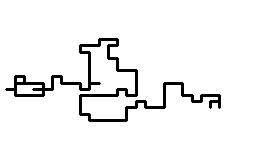
\includegraphics{domb-joyce-black-small.png}
\caption[Discrete WSAW]{Monte Carlo simulation of discrete-time WSAW with 100 steps}
\end{figure}

We let
\begin{equation}
\label{e:c}
c_T = E_0\left(e^{-U_{\gcc,\gamma,T}}\right),
	\quad
c_T(x) = E_0\left(e^{-U_{\gcc,\gamma,T}}\1_{X_T = x}\right).
\end{equation}
The \emph{two-point function} and \emph{susceptibility} are defined
as the Laplace transforms of these weights:
\begin{equation}
\lbeq{Gsa}
G_x(\gcc,\gamma,\nu)
    =
\int_0^\infty c_T(x) e^{-\nu T} \; dT
\end{equation}
and
\begin{equation}
\label{e:suscept-def}
\chi(\gcc, \gamma, \nu)
	=
\int_0^\infty c_T e^{-\nu T} \; dT
	=
\sum_{x\in\Zd} G_x(\gcc,\gamma,\nu),
\end{equation}
Note that \eqref{e:suscept-def} is more-or-less consistent with \eqref{e:susceptibility-def}
We will establish an exact analogue of \eqref{e:susceptibility-def} in Proposition~\ref{prop:finvol}.
The relationship between the two-point function for walks and spin systems will be
discussed in Section~\ref{sec:intrep}.

We also have a version of the the \emph{correlation length of order $p$}:
\begin{equation}
\label{e:clp-wsawsa}
\xi_p(\gcc, \gamma, \nu)
	=
\left(\frac{\sum_{x\in\Zd} |x|^p G_x(g, \gamma, \nu)}{\chi(g, \gamma, \nu)}\right)^{1/p}.
\end{equation}
Note that
\begin{equation}
\xi_p^p(\gcc,\gamma,\nu)
	=
\frac
{\int_0^\infty \langle |X(T)|^p \rangle c_T e^{-\nu T} \; dT}
{\int_0^\infty c_T e^{-\nu T} \; dT},
\end{equation}
where
\begin{equation}
\langle F(X) \rangle
	=
\frac{1}{c_T} E_0 (F(X) e^{-U_{g,\gamma,T}})
\end{equation}
is the expectation induced by the weights \eqref{e:c}.
Thus, $\xi_p$ is related to the Laplace transform of the mean $p$-th displacement
$\langle |X(T)|^p \rangle$.
On $\Zd$, a version of the correlation length can also be defined exactly as in \eqref{e:cl-spins}.

\begin{rk}
The discrete-time version of the WSAW-SA is straightforward to define in terms of
discrete-time simple random walk; when
$\gamma = 0$, it is known as the \emph{Domb-Joyce model} or \emph{discrete-time
weakly self-avoiding walk}. A sample of the Domb-Joyce model with 100 steps is shown
in Figure~\ref{fig:domb-joyce}. The SAW can be recovered as an
appropriate limit of the Domb-Joyce model or the continuous-time WSAW \cite{BDS12}.
\end{rk}

\subsubsection{Alternative representation}

For $f : \Zd \to \R$, let 
\begin{equation}
|\nabla f_x|^2 = \sum_{|e|=1} |\nabla^e f_x|^2,
	\qquad
|\nabla f|^2 = \sum_{x\in\Zd} |\nabla f_x|^2.
\end{equation}
Then by \eqref{e:sbp-gen}
\begin{equation}
\label{e:sbp}
\sum_{x\in\Zd} f_x \Delta f_x
	=
-\frac{1}{2} |\nabla f|^2.
\end{equation}
It follows that
\begin{equation}
\sum_{x\in\Zd} \sum_{e\in\Ucal} f_x f_{x+e}
=
2 d \sum_{x\in\Zd} f_x^2
+ \sum_{x\in\Zd} f_x \Delta f_x
=
2 d \sum_{x\in\Zd} f_x^2
- \frac{1}{2} \sum_{x\in\Zd} |\nabla f_x|^2
\end{equation}
and so we get the useful representation:
\begin{equation}
\label{e:Udef-pos}
U_{\gcc,\gamma}(f)
= (\gcc - \gamma) \sum_{x\in\Zd} f_x^2
+ \frac{\gamma}{4d} \sum_{x\in\Zd} \sum_{e\in\Ucal} |\nabla^e f_x|^2.
\end{equation}
In particular,
\begin{equation}
  \label{e:V2}
  U_{\gcc,\gamma,T} =
  (\gcc - \gamma) I_T
  + \frac{\gamma}{4d}
  |\nabla \lt_T|^2
  .
\end{equation}

%%%%%%%%%%%%%%%%%%%%%%%%%%%%%%%%%%%%%%%%%%%%%%%%%%%%%%%%%%%%%%%%%%%%%%%%%%%%%%%

\subsection{Predicted behaviour}

We can view the susceptibility \eqref{e:suscept-def} as the partition function
for a measure on walks of \emph{any} length (sometimes called a \emph{grand
ensemble}). When $\nu$ reaches the critical point
\begin{equation}
\nu_c = \nu_c(\gcc, \gamma) = \inf\{ \nu : \chi(\gcc,\gamma,\nu) < \infty \},
\end{equation}
we expect the susceptibility to diverge, which is indicative of a phase transition.
In fact, it is not clear how to show that $\chi(\gcc,\gamma,\nu_c) = \infty$ in
general, although this can be established for $\gamma = 0$
(see \cite[Lemma~\ref{log-lem:csub}]{BBS-saw4-log}). For $\gamma$
sufficiently small, this divergence will be part of our main result.

The two-point function, susceptibility, and correlations lengths of the
self-avoiding walk and (discrete- or continuous-time) WSAW-SA (with $\gamma$ small
depending on $\gcc$) on $\Zd$ are all expected
to scale according to analogues of \eqref{e:Gpred}--\eqref{e:xippred}.
Moreover, the discussion in Section~\ref{sec:asymp} suggests that
\begin{align}
\label{e:cT-asymp}
c_T                       &\sim C_5 e^{-\nu_c T} T^{-\gammabar}, \\
\label{e:XT-asymp}
\langle |X_T|^2 \rangle   &\sim C_6 T^{-\nubar}.
\end{align}
The critical exponents $\gammabar, \nubar, \eta$ are expected to be universal;
in particular, they should only depend on $d$ in this context.

Below, we discuss the predicted values of the exponents for $\gamma$ small before
turning our attention to the case of large $\gamma$. A more detailed reference is
\cite{MS93}. The values of $\nubar$ were first predicted\footnote{Flory's prediction
for $d = 3$ is no longer generally accepted.} by the chemist Paul Flory \cite{Flor49}, who
later won the 1974 Nobel Prize in Chemistry for his work on polymers.

\subsubsection{Dimension $d = 1$}

For the SAW, dimension $1$ is trivial: the only self-avoiding walks are straight
lines. This is not the case for the WSAW, see e.g.\ the survey \cite{HK01}.

\subsubsection{Dimension $d = 2$}

In $d = 2$, the predicted values of the critical exponents are
\begin{equation}
\nubar = 3/4, \quad \gammabar = 43/32, \quad \eta = 5/24.
\end{equation}
It was shown in \cite{LSW04} that the scaling limit of SAW, if it exists and
is conformally invariant, is given by $\SLE_{8/3}$, which is consistent with
the predicted exponents given above.

It is not immediately clear how to make sense of the supercritical regime
($\nu < \nu_c$ for WSAW-SA).
However, the authors of \cite{LSW04} considered SAW on a discretized bounded
planar domain. They showed that the scaling limit of supercritical
SAW conditioned to start and end on the boundary of the domain is space-filling
(their results extend to all dimensions $d \ge 2$).

\subsubsection{Dimension $d = 3$}

In $d = 3$, again very little is known. Only numerical approximations for
the critical exponents are available.

\subsubsection{Dimension $d > 4$}

The upper-critical dimensions for these models is $d = 4$ and the mean-field
exponents are the same as for models in the Ising universality class, namely
$\gammabar=1$, $\nubar = 1/2$, $\eta = 0$. In other words, self-avoiding walk
is expected to scale like simple random walk in dimensions above $4$.

Brydges and Spencer introduced the lace expansion in \cite{BS85} and used it
to show that $\nubar = 1/2$ if $d > 4$ for the discrete-time WSAW.
By vastly extending this method, Hara and Slade \cite{HS92a,HS92b} showed for the
SAW that $\gamma = 1$, $\nubar = 1/2$ (for the mean-squared displacement, correlation
length, and correlation length of order $2$), $\eta = 0$, and the scaling limit
is Brownian motion.

Even above the upper-critical dimension, very little is known about WSAW-SA with
$\gamma \ne 0$. Exceptions include \cite{HH17,Uelt02}.

\begin{rk}
\label{rk:bubble}
Define the free \emph{bubble diagram} to be the $\ell^2(\Zd)$ norm of the massive
Green function $x \mapsto C_{0x}$. Thus, by
\eqref{e:greendef}, if $z = 2 d / (m^2 + 2 d)$, then
\begin{equation}
\label{e:bubble-def}
B_{m^2}
	=
\|C\|_{\ell^2(\Zd)}
	=
(m^2 + 2 d)^{-2} \sum_{m,n=0}^\infty z^{m+n} \Pr(X_m = Y_n),
\end{equation}
where $X$ and $Y$ are independent simple random walks started at $0$. In other words,
$B_{m^2}$ is proportional to the expected number of intersections between the traces of two
such random walks \emph{killed} at rate $1 - z$. The upper-critical dimension can
be ``guessed'' as follows. First, we make the convenient definitions
\begin{equation}
\label{e:bubble}
{\sf B}_{m^2} = (n + 8) B_{m^2},
	\quad
{\sf b} = \frac{n + 8}{16\pi^2}.
\end{equation}
Then it is an exercise in Fourier analysis to show that in the limit $m^2\downarrow0$
(equivalently, $z\uparrow1$)
\begin{equation}
\label{e:bubble-log}
{\sf B}_{m^2}
	\sim
\begin{cases}
{\sf b} \log m^{-2},
	&
d = 4
	\\
{\sf B}_0,
	&
d > 4.
\end{cases}
\end{equation}
\end{rk}

\subsubsection{Dimension $d = 4$}

As discussed in Section~\ref{sec:rg-intro}, Bauerschmidt, Brydges, and Slade have
recently made great strides in the case $d = 4$ using a renormalisation group method.
One of the novelties of this method, besides its applicability to multi-component
spin systems, is that it can be used to study the WSAW via an integral representation
we will discuss in Section~\ref{sec:intrep}. This method was first applied to walks
in \cite{BBS-saw4-log,BBS-saw4}, where the susceptibility and two-point function were
studied.

\subsubsection{Phase diagram}

Let $d \ge 2$. The predicted behaviour of self-avoiding walk with attraction is discussed
in \cite{Vand98}.
When $\gamma$ reaches the $\theta$-curve in Figure~\ref{fig:theta-curve}, it is predicted
that the value of $\nubar$ changes discontinuously to $\nubar_\theta = 4/7$ if $d = 2$
and $\nubar_\theta = 1/2$ if $d \ge 3$. The predicted values for $\nubar$
in the other regions of the phase diagram are shown in the figure. In particular, for
$\gamma > \beta$, the WSAW-SA is expected to undergo a collapse transition ($\nubar = 0$).
This has recently been shown for a model of prudent self-avoiding walk with self-attraction
in \cite{PT16}.

\begin{figure}
\centering
\includegraphics{theta_curve}
\caption[Phase diagram of WSAW-SA]{Phase diagram for the WSAW-SA}
\label{fig:theta-curve}
\end{figure}
